% autor: Ondrej Lukasek (xlukas15)
% datum: 10.12.2023
% licence: GNU GPL V3

\documentclass[11pt, a4paper]{article}

\usepackage[left=2cm,text={17cm, 24cm},top=3cm]{geometry}
\usepackage[utf8]{inputenc}
\usepackage[czech]{babel}
\usepackage{times}
\usepackage[hidelinks, unicode]{hyperref}
\usepackage{breakurl}
\usepackage{graphicx}
\def\UrlBreaks{\do\/\do-}

\setlength{\parindent}{\baselineskip}
\setlength{\parskip}{0em}

\begin{document}

\begin{titlepage}
    \begin{center}
        \Huge \textsc{Vysoké učení technické v~Brně}\\
        \huge \textsc{Fakulta informačních technologií}\\
        
        \vspace{\stretch{0.382}}
        
        {\LARGE Modelování a simulace -- Technická zpráva\\
        \Huge T8: CA v dopravě}
        
        \vspace{\stretch{0.618}}
    \end{center}
    
    {\Large \today \hfill Ondřej Lukášek (xlukas15)}
\end{titlepage}

\tableofcontents
\newpage

\section{Úvod}

Tato práce řeší projekt zaměřený na implementaci a simulaci modelu parkoviště. Projekt byl vyvíjen v rámci kurzu Modelování a Simulace. Cílem projektu je ukázat, jak parkování a strategie řidičů ovlivňují využití parkovacích ploch u obchodních domů. 

Pomocí experimentů je v práci zkoumáno, jak různé konfigurace parkovišť s chováním řidičů ovlivňují efektivitu a využití parkovacích ploch.

\subsection{Účastníci a zdroje}
\label{ucastnici}

Autorem tohoto projektu je Ondřej Lukášek, student Fakulty informačních technologií Vysokého učení technického v Brně.

Pro vypracování projektu bylo využito článků a výzkumů z oblasti parkování u obchodních domů. Dále byly získány informace o průměrné vytíženosti obchodního domu, prostřednictvím jednoho ze zaměstnanců. To přispělo k možnosti přesnější simulace vytíženosti parkovacích ploch.

Všechny použité zdroje a odkazy jsou dostupné na konci tohoto dokumentu v části Použité zdroje, na straně~\pageref{zdroje}.

\subsection{Prostředí a validace}

Vývoj byl prováděn za využití jazyka C, který umožňuje efektivně implementovat a simulovat celulární automaty.

% TODO - mozna pridat nejake odkazy na konkretni obchodni domy, ktere byly prikladem
Simulace a experimenty byly prováděny pod různými konfiguracemi, aby odrážely reálné scénáře parkování. Validita byla ověřena pomocí snímků\footnote{Snímky byly prohlíženy na \url{https://www.google.com/maps/}, platných k 9.12.2023.} reálných parkovišť přilehlých u obchodních domů, čímž se zjistilo, že simulované parkoviště věrně napodobuje své reálné předlohy, čímž jsou využitelné v praxi, případně je možné je snadno upravit podle individuálních požadavků.

\section{Rozbor tématu a použitých metod/technologií}

Tato kapitola detailně popisuje rozbor systému parkování a obsahuje v sobě popis metod a technologií pro jeho modelování a simulaci.

\subsection{Použité postupy}

Model parkoviště a chování řidičů bylo vytvořeno na základě nastudovaných principů celulárních automatů~\cite{Peringer_2023}, za využití Von Neumannova okolí, které bylo ideální pro hledání místa na parkovišti.

Samotné parkoviště je dále implementováno pomocí dvourozměrného pole o proměnlivé velikosti podle toho, což umožňuje dále ladit simulaci tak, aby se co nejvíce vyoptimalizovalo vytížení parkoviště a nebylo moc velké, případně moc malé. Je to důvodu, že v dvourozměrném poli se lze dobře orientovat pomocí souřadnic a není potřeba pracovat s nějakými složitými strukturama, čímž se toto řešení jeví jako nejideálnější.

Průměrné parkovací časy byly vybrány na základě již provedených výzkumů~\cite{Arndt_Gronmo_1977}~\cite{Bawa_Sinha_Kant_2019}~\cite{Rodgers_2023}, což zlepšuje validitu celého modelu, nicméně jsou přebrány z různých částí světa, tudíž je pro lokální využití vhodnější využít soukromé průzkumy uživatele.

Typy řidičů, které jsou implementovány v programu jsou převzaté z praxe, aby jejich chování více zpřes\-ňo\-va\-lo simulační model. Některým řidičům nezáleži na tom, zda parkují blízko jiných. Někteří chtějí okolo sebe při parkování více místa, jiní zase místo kolem sebe vyloženě vyžadují.

\subsection{Použité technologie}

Pro vytvoření simulačního modelu bylo využito jazyka C, spolu s využitím některých z jeho standardních knihoven\footnote{stdio, stdlib, time, stdbool, unistd. Seznam všech standardních knihoven s jejich popisy je zde: \url{https://en.cppreference.com/w/c/header}}.

Auta jsou implementována formou struktury, obsahující důležité informace, jako čas příjezdu, odjezdu, a podobně. Struktury jsou v jazyce C běžně využívané.

Kromě výše zmíněného dvourozměrného pole bylo také využito jednosměrně vázaného seznamu~\cite{pinkikrjad_2023} pro vytvoření seznamu vozidel, která jsou aktuálně obsažena v systému.

\section{Koncepce}

Tato kapitola se zaměřuje na abstrakci reality do formy modelu a popisuje, jak se promítly vlastnosti reálného světa do simulačního modelu.

\subsection{Způsob vyjádření modelu}

Model parkování je reprezentován dvourozměrným celulárním automatem, jehož základní strukturu lze vidět na Obrázku \ref{parking_lot}. Každé parkovací místo je reprezentováno jako buňka v mřížce, která může nabývat dvou různých stavů: obsazeno (\texttt{true}), volno (\texttt{false}). Způsob parkování řidičů je modelován pomocí pravidel, která jsou se aplikují na určitá místa, na základě buněk parkoviště (parkovacích míst) a jejich okolí.

Obsazení parkoviště se neustále mění. Auta na parkoviště přijíždějí (tyto časy jsou převzaty z podkladů získaných od jednoho ze zaměstanců obchodního domu, jak je zmíněno v kapitole \ref{ucastnici}) a odjíždějí v různé časy (auta parkují na parkovišti různou dobu ~\cite{Arndt_Gronmo_1977}~\cite{Bawa_Sinha_Kant_2019}~\cite{Rodgers_2023}), což napomáhá větší autentičnosti modelu.

\begin{figure}[ht]
  \centering
  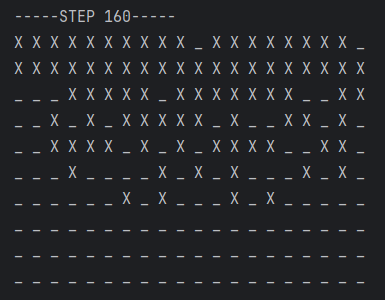
\includegraphics[width=0.5\textwidth]{img/parking_lot.png}
  \caption{Dvourozměrný model parkoviště}
  \label{parking_lot}
\end{figure}

\subsection{Popis konceptuálního modelu}

V tomto modelu jsou parkovací místa buňky, které v čase mění svůj stav podle toho, kde v parkovišti se nacházejí a kdy přijíždějí o odjíždejí vozidla, snažící se zaparkovat na parkovací ploše, a jaký je aktuální typ tohoto vozidla.

Model bere v úvahu různé typy vozidel (respektive jejich řidičů) a jejich preference při parkování. Typ vozidla je generován při příjezdu do systému na základě pravděpodobnostního určení. Zároveň vozidla zahrnuje i nějakou trpělovist řidiče, která je vyjádřená v parkovacích pokusech, které je schopné vozidlo uskutečnit. Pokud se nepodaří vozidlu zaparkovat do jemu individuálně vygenerovanému počtu pokusů, poté se mohou jeho pravidla parkování změnit (vizte senzam typů vozidel v kapitole \ref{driver_types}), případně opouštějí systém. Typy vozidel jsou následující: 

\label{driver_types}
\begin{enumerate}
    \item Zkušený řidič - vyhledává jakékoliv jedno volné místo, pokud možno co nejblíže vchodu do obchodního domu. Nezáleží na tom, jak vypadají místa okolo.
    \item Opatrný řidič - vyhledává parkovací místo na základě toho, jestli je vedle volného parkovacího místa volné ještě jedno. Pokud ano, potom tam zaparkuje. Pokud se mu nepodaří na parkovišti zaparkovat, na svůj poslední parkovací pokus zaparkuje na jakékoli volné místo, co nejblíže ke vchodu.
    \item Nový řidič - vyhledává alespoň 3 volná místa vedle sebe a parkuje do prostředního z nich. Pokud se mu ani v jednom z jeho parkovacích pokusů nepodaří zaparkovat, opouští systém.
\end{enumerate}

Neopomenutelnou součátí modelu je také způsob, jakým jsou vozidla generována a odstraňována ze sys\-té\-mu, což odpovídá realistickému příjezdu a odjezdu vozidel v reálném světě, přičemž tyto údaje o parkování vy\-chá\-ze\-jí z reálných průzkumů~\cite{Arndt_Gronmo_1977}~\cite{Bawa_Sinha_Kant_2019}~\cite{Rodgers_2023}. Tento aspekt modelu je zásadní pro simulaci skutečných podmínek parkování a umožňuje analýzu vlivu různých faktorů, jako je velikost parkoviště, na celkovou efektivitu, kapacitu a zatížení parkovací plochy.

% TODO tady by se mozna hodil obrazek nejakeho automatu, jak ridici prijizdi na parkoviste, snazi se zaparkovat, jak odjizdi.

\section{Architektura simulačního modelu/simulátoru}

Tato kapitola se zaměřuje více konkrétně na technické prvky simulačního modelu a především tomu, jak je konceptuální model mapován do konkrétních forem simulátoru.

\subsection{Mapování konceptuálního modelu do simulátoru}

Model ve svém základu pracuje se strukturou parkoviště, pro kterou je alokována pamět a je inicializována funkcí \texttt{initializeParkingLot()}, na konci programu je alokovaná paměť uvolněna pomocí funkce pro vyčištění paměti \texttt{clearParkingLot()}.

\bigskip

\noindent Následně se spustí simulace v čase, která probíhá podle počtu zvolených kroků simulace, kdy jeden krok odpovídá přibližně jedné minutě reálného světa. Dobu simulace si může uživatel nastavit pomocí argumentů příkazové řádky (kapitola \ref{arguments}).

V každém kroku simulace se v systému generuje náhodný počet aut od 3 do 4 v průměru. To vychází ze získaných informací od jednoho ze zaměstnanců (kapitola \ref{ucastnici}), který sdělil, že jedním z obchodních domů\footnote{Jedná se konkrétně o Kaufland Kuřim, na ulici Blanenská} projde za den přibližně mezi 2700 až 3100 zákazníky, což přibližně odpovídá 3-4 autům za minutu při otevírací době 7-22 hodin ($ 7-22=15 $ otevíracích hodin, $ 15 * 60 = 900 $ otevíracích minut, což znamená $ 2700 / 900 = 3 $ až $ 3300 / 900 \approx 3.67 \approx 4 $ auta za minutu). 

Každému z aut se při vygenerování přiřadí náhodně typ (vizte kapitolu \ref{driver_types}), maximální počet pokusů pro zaparkování (což signalizuje trpělivost řidiče). Dále se zapíše čas příjezdu (ve kterém čase simulace přijelo auto do systému) a jak dlouho bude v systému setrvávat, pakliže se mu podaří zaparkovat (doba parkování je vybrána náhodně podle časů získaných z průzkumů ~\cite{Arndt_Gronmo_1977}~\cite{Bawa_Sinha_Kant_2019}~\cite{Rodgers_2023}).

Zároveň se také při každém generování auta inkermentuje počítadlo aut, která přijela, což je užitečné pro získání statistik.

\bigskip

\noindent Po příjezdu vozidel do systému se vozy pokusí postupně zaparkovat (funkce \texttt{attemptToPark()}, která dále volá funkci \texttt{parkCar()}). Vozidla mohou mít různé typy, které jsou detailněji popsány v kapitole \ref{driver_types} a typ vozu definuje pravidla, kterými se bude při parkování řídit. Pokud se autu nepodaří zaparkovat, inkrementuje se jeho počítadlo pokusů o zaparkování. Pokud se zaparkovat podaří, potom se buňka (souřadnice) parkoviště nastaví jako obsazená (\texttt{true}) a ve struktuře auta se proměnná \texttt{parked} nastaví na \texttt{true}.

\bigskip

\noindent Následně program projde seznam všech vozidel (funkce \texttt{updateCars()}) a vyřadí ze seznamu všechna vozidla, kterým vypršel čas, který jim byl vyhrazen na parkovací dobu. Také jsou ze seznamu (a tedy i ze systému) vyřazena všechna auta, která přesáhla svůj maximální počet pokusů o zaparkování.

V této funkci se také inkrementuje počítadlo aut, kterým se nepodařilo zaparkovat, avšak inkrementuje se pouze v případě, kdy nějaké z vozidel přesáhlo svůj maximální počet pokusů o zaparkování. Toto počítadlo je důležité pro koncové statistiky, protože podá informaci o tom, kolika vozidlům se vůbec zaparkovat nepodařilo, a tak je možné zkusit příští běh simulace s jinými parametry (například s velikostí parkoviště)(vizte kapitolu \ref{arguments}).

\bigskip

\noindent Každých 10 běhů simulace se také spustí funkce \texttt{printStatus()}, která vykreslí aktuální stav parkoviště na standardní výstup programu (vizte Obrázek \ref{parking_lot}). Na obrázku znázorňuje znak \texttt{X}, že je parkovací místo obsazené. Znak \texttt{\_} zase znázorňuje, že místo je volné.

\bigskip

\noindent Po proběhnutí všech kroků simulace se na standardní výstup vypíší statistiky pomocí funk\-ce \texttt{printStats()}. Mezi tyto statistiky patří konfigurace parkoviště (celkový počet míst, počet řádků, počet sloupců), počet vozidel, která vstoupila do systému, počet vozidel, kterým se v průběhu simulace nepodařilo zaparkovat a opustila systém předčasně, a počet aut, kterým se zaparkovat podařilo. Příklad tabulky statistik lze vidět na obrázku \ref{statistics}.

\begin{figure}[ht]
  \centering
  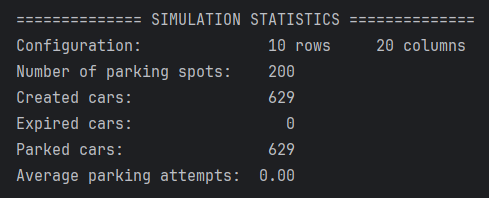
\includegraphics[width=0.6\textwidth]{img/statistics.png}
  \caption{Příklad tabulky statistik}
  \label{statistics}
\end{figure}

\subsection{Argumenty příkazové řádky}
\label{arguments}

Program umožňuje rychlé nastavení klíčových prvků simulace, jako je počet kroků simulace, konfigurace parkoviště (nastavení počtu řádků a sloupců), nastavení vchodu do obchodního domu (určí se, které parkovací místo z prvního řádku je ke vchodu nejblíže), což umožňuje větší flexibilitu a použitelnost pro různé obchodní domy. Nakonec je také program schopen vypsat nápovědu k jeho využití.

\begin{itemize}
    \item \emph{-s} -- počet kroků simulace (celé, kladné číslo). Pokud není zadáno, je v základu nastaveno 180 kroků (3 hodiny).
    \item \emph{-r} a \emph{-c} -- počet řádků a sloupců parkovací plochy (celé, kladné číslo). Musí být zadány oba současně. Pokud nejsou zadány, konfigurace parkoviště je základně 10 řádků a 20 sloupců.
    \item \emph{-e} -- vstup na parkoviště (celé, kladné číslo). Označuje sloupec v prvním řádku parkovacích míst, ke kterému je vstup nejblíže. Pokud není zadán, vstup do obchodního domu je nastaven na střed, což znamená $ pocet\_sloupcu / 2 $.
    \item \emph{-h} -- Vypíše nápovědu na standardní výstup, pokud je zadán.
\end{itemize}

\section{Podstata simulačních experimentů a jejich průběh}
\label{experiment_goals}

Cílem následujících experimentů je optimalizovat rozměry parkoviště pro scénář, kde v průměru přijíždí 3-4 auta za simulační krok v simulaci trvající 15 hodin a dobu setrvání na prakovišti 20-40 minut, jako to odpovídá realitě. Experimenty byly zaměřeny na zjištění, jaké rozměry parkoviště nejlépe vyhovují těmto podmínkám a jak se parkoviště chová v různých konfiguracích.

\subsection{Postup experimentování}

Experimenty byly postaveny na postupném upravování rozměrů parkoviště a sledování efektivity parkování vozidel. Začalo se s výchozími rozměry (tedy 10 řádků a 20 sloupců), které byly postupně měněny s cílem zvýšit efektivitu využití prostoru, zkrátit dobu hledání volného místa pro přijíždějící vozidla a pokud možno eliminovat množství aut, kterému se nepodařilo zaparkovat. Zároveň ale žádoucí, aby parkovací plocha nebyla příliš velká, protože nákup jakékoli plochy je nákladný. V každém experimentu bylo zaznamenáno, kolik aut úspěšně zaparkovalo, kolik opustilo systém kvůli neúspěšnému hledání parkovacího místa a jak dlouho trvalo najít místo. Také byl každý experiment proveden třikrát a byly z něj zaznamenány grafy pro každou hodinu běhu. Grafy byly generovány v jazyce Python za použití knihovny matplotlib~\cite{Kumar_2023}.

\newpage

\subsection{Dokumentace experimentů}

\subsubsection{Výsledky se základními parametry \texorpdfstring{$10 \times 20$}{10 x 20}}
\label{experiment1}

Tento experiment proběhl bez jakýchkoliv potíží, každému vozidlu se podařilo zaparkovat na první pokus a u žádného z nich se nestalo, že by odešlo ze systému na základě vyprchaného počtu pokusů o zaparkování. Po extrakci průměrných množství zaparkovaných aut z Obrázku \ref{exp1} vychází, že v průměru se na parkovišti nacházelo 105 aut.

Lze tedy usoudit, že parkoviště je možné ještě optimalizovat a trochu zmenšit, proto se v dalším experimentu parkoviště zmenší ve svém rozměru.

\begin{figure}[ht]
  \centering
  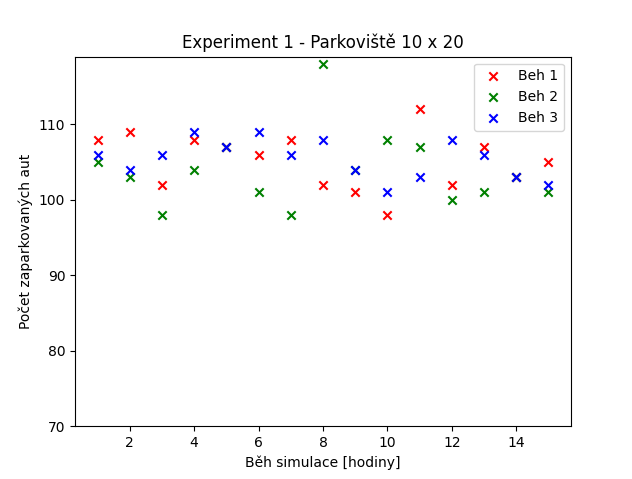
\includegraphics[width=0.6\textwidth]{img/exp1.png}
  \caption{Experiment se základními parametry}
  \label{exp1}
\end{figure}

\newpage

\subsubsection{Výsledky parkoviště \texorpdfstring{$8 \times 15$}{8 x 15}}
\label{experiment2}

Zde byly výsledky poměrně nepříznivé. Oproti předchozímu experimentu bylo míst výrazně méně. Z 200 míst se počet snížil na pouhých 120. To se také výrazně promítlo na obsazených místech parkoviště. Obsazená místa nyní v žádném z experimentů nepřesáhla 100 míst (vizte Obrázek \ref{exp2}), protože průměrně byly ze 120 míst obsazeno pouhých 90 míst.

Také by bylo na místě si nyní zmínit průměrný počet aut, která byla v systému vytvořena. Těch bylo v průměru ze všech 3 běhů 3148. Z těchto aut v průměru nezaparkovalo 462, což znamená, že přibližně 14.67\% aut na parkovišti vůbec nezaparkovalo.

Lze tedy jednoznačně usoudit, že parkoviště musí být opět o něco zvětšeno v dalším experimentu.

\begin{figure}[ht]
  \centering
  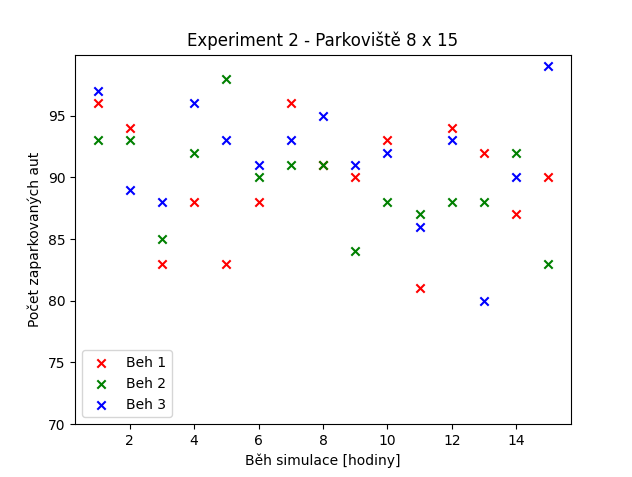
\includegraphics[width=0.6\textwidth]{img/exp2.png}
  \caption{Experiment s rozměry $8 \times 15$}
  \label{exp2}
\end{figure}

\newpage

\subsubsection{Výsledky parkoviště \texorpdfstring{$10 \times 17$}{10 x 17}}
\label{experiment3}

V tomto experimentu byly oproti předchozímu výsledky opět o něco příznivější (jak se dalo očekávat). Počet vozidel na parkovišti znovu běžně překračoval 100 a průměrně množství zaparkovaných aut v simulaci bylo 104 (vytížení v jednotlivých hodinách lze pozorovat na Obrázku \ref{exp3}).

Nicméně se ani zde nejedná o naprosto přesvědčivý výsledek, protože průměrně se za jeden běh nepodařilo vůbec zaparkovat 5 vozidlům, což je přibližně 0.16\% ze všech aut v systému. Toto číslo stále není v naprostém souladu s cílem těchto experimentů (vizte kapitolu \ref{experiment_goals}), a je tedy potřeba parkoviště ještě o něco zvětšit, nicméně už to stačí jen velmi málo, aby byla úspěšnost zaparkování 100\%.

\begin{figure}[ht]
  \centering
  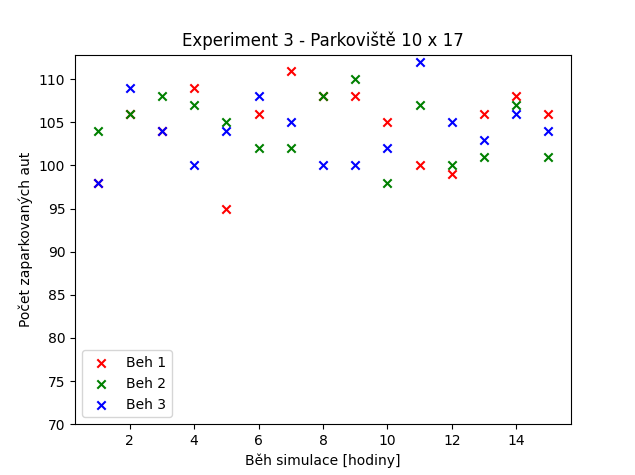
\includegraphics[width=0.6\textwidth]{img/exp3.png}
  \caption{Experiment s rozměry $10 \times 17$}
  \label{exp3}
\end{figure}

\newpage

\subsubsection{Výsledky parkoviště \texorpdfstring{$10 \times 18$}{10 x 18}}
\label{experiment4}

Tento experiment už se jeví jako ideální, protože se opět, stejně jako v prvním experimentu (kapitola \ref{experiment1}), podařilo zaparkovat všem vozidlům, která vstoupila do systému. Těchto vozidel bylo v průměru za jeden běh 3149 (vytíženost v jednotlivých hodinách lze vidět na Obrázku \ref{exp4}).

Na první pohled jsou čísla velice podobná, jako při prvním experimentu, protože je parkovací plocha zúžená o pouhé 2 sloupce. Nicméně to při průměrné velikosti parkovacího místa $5 \times 2,3$ metrů čtverečních~\cite{France_2022} dělá ušetření přibližně 230 čtverečních metrů, což není při ceně stavební plochy malý rozdíl.

\begin{figure}[ht]
  \centering
  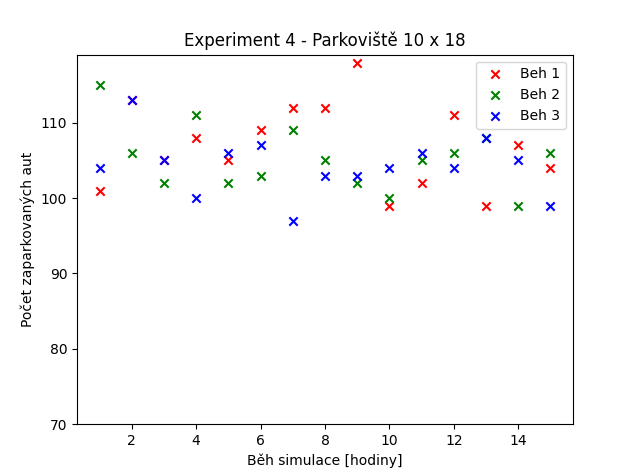
\includegraphics[width=0.6\textwidth]{img/exp4.png}
  \caption{Experiment s rozměry $10 \times 18$}
  \label{exp4}
\end{figure}

\newpage

\subsection{Závěry experimentů}

Celkově byly provedeny 4 experimenty. Všechny byly odsimulovány s různou konfigurací parkoviště a postupně se blížily k ideálnímu výsledku, stanoveném v kapitole \ref{experiment_goals}. K tomuto výsledku se došlo v posledním, čtvrtém experimentu (kapitola \ref{experiment4}), který se svou konfigurací demonstroval ideální výsledky.

\section{Shrnutí simulačních experimentů a závěr}

Zjištění z výsledků simulačních experimentů ukazují, že parkoviště o rozměrech $10 \times 18$ poskytuje nejlepší vyváženost mezi kapacitou a efektivním využitím prostoru. Tento výsledek je relevantní zejména pro lokace, kde je jedním ze stěžejních úkolů efektivní vytížení omezených prostor.

Program by bylo možné i nadále ladit a upravovat. Například by v případě reálného využití v praxi zá\-kaz\-ní\-kem bylo vhodné, aby byly do programu implementovány hodnoty jeho vlastních průzkumů, neboť tento simulační model funguje na obecné rovině, která vychází z veřejných zdrojů (ty jsou shrnuté v kapitole \ref{zdroje}). Doplnění hodnot a úprava programu na základě vlastních soukromých šetření by přispěla k jeho největší přesnosti pro individuální využití.

\newpage

\bibliographystyle{czechiso}
\renewcommand{\refname}{Použité zdroje}
\bibliography{ims_sources}
\label{zdroje}

\end{document}